\documentclass[titlepage]{article}
\usepackage[subpreambles=true]{standalone}
\usepackage{twemojis}
\usepackage{graphicx} % Required for inserting images
\usepackage{amsmath}
\usepackage{amssymb}
\usepackage{hyperref}       % hyperlinks
\usepackage{url}            % simple URL typesetting
\usepackage{booktabs}       % professional-quality tables
\usepackage{amsfonts}       % blackboard math symbols
\usepackage{nicefrac}       % compact symbols for 1/2, etc.
\usepackage{microtype}      % microtypography
\usepackage[table,xcdraw,dvipsnames]{xcolor}
\usepackage{enumitem}
\usepackage{natbib}
\usepackage{algorithm2e}
% \usepackage{algpseudocode}
\usepackage{pifont}
\usepackage{soul}
\usepackage{phoenician}
\usepackage{bbm}
\usepackage{wrapfig}
\usepackage[nameinlink]{cleveref}
\usepackage[a4paper, left=2.5cm, right=2.5cm, top=2.5cm, bottom=2.2cm]{geometry}
\usepackage[skins,theorems,many]{tcolorbox}
\definecolor{code_bg}{rgb}{0.97,0.85,0.7}
\definecolor{dodgerblue}{HTML}{027BCE}
\definecolor{royalblue}{HTML}{0e6ba8}
\definecolor{orange}{HTML}{f8961e}
\definecolor{lightgreen}{HTML}{74c476}
\definecolor{forestgreen}{HTML}{005a32}
\definecolor{purple}{HTML}{5f0f40}
\definecolor{red}{HTML}{bf0603}
\definecolor{darkred}{HTML}{780000}
\definecolor{bordeaux}{HTML}{7F1734}
\definecolor{teal}{HTML}{006d77}
\hypersetup{
    colorlinks=true,
    linkcolor=red,     % Internal links (sections, etc.)
    citecolor=dodgerblue,     % Citations
    urlcolor=dodgerblue        % External URLs
}
\usepackage{import} % Allows scoped imports
\usepackage{amsthm}
\usepackage{tikz}
\definecolor{MSBlue}{rgb}{.204,.353,.541}
\definecolor{MSLightBlue}{rgb}{.31,.506,.741}
% Define a new fontfamily for the subsubsection font
% Don't use \fontspec directly to change the font


% \usepackage{cmbright}
% \tikzset{every picture/.style={font=\fontfamily{cmbright}\selectfont}}
\usepackage{minted}
\usemintedstyle{colorful}
\setminted{
    bgcolor=orange!15
}
% \usemintedstyle{fruity}
\usetikzlibrary{arrows.meta}
\usetikzlibrary{shapes.geometric, fit, positioning}

\newtheoremstyle{cleanremark}
  {\topsep}                    % Space above
  {\topsep}                    % Space below
  {\normalfont}                % Body font (Remarks are usually upright text)
  {}                           % Indent amount
  {\bfseries}                  % Theorem head font (e.g., Bold "Remark 3.6")
  {}                           % Punctuation after theorem head (LEAVE EMPTY to remove trailing periods)
  {.5em}                       % Space after theorem head
  {}                           % Theorem head spec (can be left empty)

% Apply your clean style
\theoremstyle{cleanremark}
\newtheorem{corollary}{Corollary}[section]
\newtheorem{remark}{Remark}[section]

\tcbset{highlight math style={enhanced,
  colframe=orange,colback=orange!40,arc=4pt,boxrule=1pt}}

%%%% FOR THE NIGHT TIME/LATE HOURS !!
% \pagecolor[HTML]{282A36} %black
% \color[rgb]{0.8,0.8,0.8} %grey
%%%%%
\renewcommand{\qedsymbol}{\textit{End of proof.}}
\renewcommand{\qed}{\newline\qedsymbol}%
\tcbuselibrary{theorems}
\newtcbtheorem
  [number within=section]% init options
  {definition}% name
  {Definition}% title
  {%
    colback=red!25,
    colframe=bordeaux,
    fonttitle=\large \bfseries,
    width=0.9\linewidth, 
    center
  }% options
  {def}% prefix
\crefname{tcb@cnt@definition}{Definition}{Definitions}
\Crefname{tcb@cnt@definition}{Definition}{Definitions}

\newtcbtheorem
  [number within=section]% init options
  {theorem}% name
  {Theorem}% title
  {%
    colback=royalblue!35,
    colframe=royalblue,
    fonttitle=\large \bfseries,
    width=0.9\linewidth, 
    center
  }% options
  {th}% prefix
\crefname{tcb@cnt@theorem}{Theorem}{Theorems}
\Crefname{tcb@cnt@theorem}{Theorem}{Theorems}

\newtcbtheorem
  [number within=section]% init options
  {note}% name
  {Note}% title
  {%
    colback=forestgreen!25,
    colframe=forestgreen!85,
    fonttitle=\large \bfseries,
    width=0.9\linewidth, 
    center
    }% options
  {}% prefix
\crefname{tcb@cnt@note}{Note}{Notes}
\Crefname{tcb@cnt@note}{Note}{Notes}

\newtcbtheorem
  [number within=section]% init options
  {summary}% name
  {Summary}% title
  {%
    colback=purple!25,
    colframe=purple!95,
    fonttitle=\large \bfseries,
    width=0.9\linewidth, 
    center
    }% options
  {}% prefix
\crefname{tcb@cnt@summary}{Summary}{Summaries}
\Crefname{tcb@cnt@summary}{Summary}{Summaries}

\newtcbtheorem
  [number within=section]% init options
  {example}% name
  {Example}% title
  {%
    colback=teal!25,
    colframe=teal!95,
    fonttitle=\large \bfseries,
    width=0.9\linewidth,
    breakable,
    enhanced,                
    center
    }% options
  {}% prefix
\crefname{tcb@cnt@example}{Example}{Examples}
\Crefname{tcb@cnt@example}{Example}{Examples}

\crefname{equation}{Eq.}{Eqs.}
\Crefname{equation}{Eq.}{Eqs.}
\crefname{figure}{Figure}{Figures}
\Crefname{figure}{Figure}{Figures}
\crefname{corollary}{Corollary}{Corollaries}
\Crefname{corollary}{Corollary}{Corollaries}
\crefname{remark}{Remark}{Remarks}
\Crefname{remark}{Remark}{Remarks}

%% Add bibliography %%
\usepackage{filecontents}

\begin{filecontents}{references.bib}
@misc{A01,
  author = {Author, A.},
  year = {2001},
  title = {Alpha},
}
\end{filecontents}

%%%%%%%%%%%%%%%%%%%%%%%%%% NEW COMMANDS FOR FAST MATHS %%%%%%%%%%%%%%%%%%%%%%%%%%%%%%%%%%%%%%%%%%%%% 
\newcommand{\pcondsrc}{p_{\text{src}}(\mathbf{x}_{\text{src}}\mid \theta)}
\newcommand{\pcondtgt}{p_{\text{tgt}}(\mathbf{x}_{\text{tgt}}\mid \theta)}
\newcommand{\src}{\text{src}}
\newcommand{\tgt}{\text{tgt}}
\newcommand{\psrc}{p_{\text{src}}(\mathbf{x}_{\text{src}})}
\newcommand{\emptypsrc}{p_{\text{src}}}
\newcommand{\emptyptgt}{p_{\text{tgt}}}
\newcommand{\pbbsrc}{\mu_{\text{src}}}
\newcommand{\pbbtgt}{\mu_{\text{tgt}}}
\newcommand{\ptgt}{p_{\text{tgt}}(\mathbf{x}_{\text{tgt}})}
\newcommand{\xsrc}{\mathbf{x}_{\text{src}}}
\newcommand{\xtgt}{\mathbf{x}_{\text{tgt}}}
\newcommand{\wtwo}{$\mathcal{W}_2$}
\newcommand{\kl}{\text{KL}}
\newcommand{\indcp}{\mu_{\text{src}} \otimes \mu_{\text{tgt}}}
% \newcommand{\mathbf{I}}{\mathbbm{1}}
\usepackage{pgffor} % Required for the loop

\foreach \l in {a,b,c,d,e,f,g,h,i,j,k,l,m,n,o,p,q,r,s,t,u,v,w,x,y,z}{%
    \expandafter\xdef\csname bb\l\endcsname{\noexpand\mathbb{\uppercase{\l}}}%
}
\DeclareMathOperator{\sech}{sech}
\DeclareMathOperator{\csch}{csch}


%%%%%%%%%%%%%%%%%%% MAIN PAGE %%%%%%%%%%%%%%%%%%%%%%%%%%%%%%
\title{\huge Introduction à l'Intelligence Artificielle (IA) \\ et à l'Apprentissage Machine (ML) \\ pour lycéen(ne)s \\ 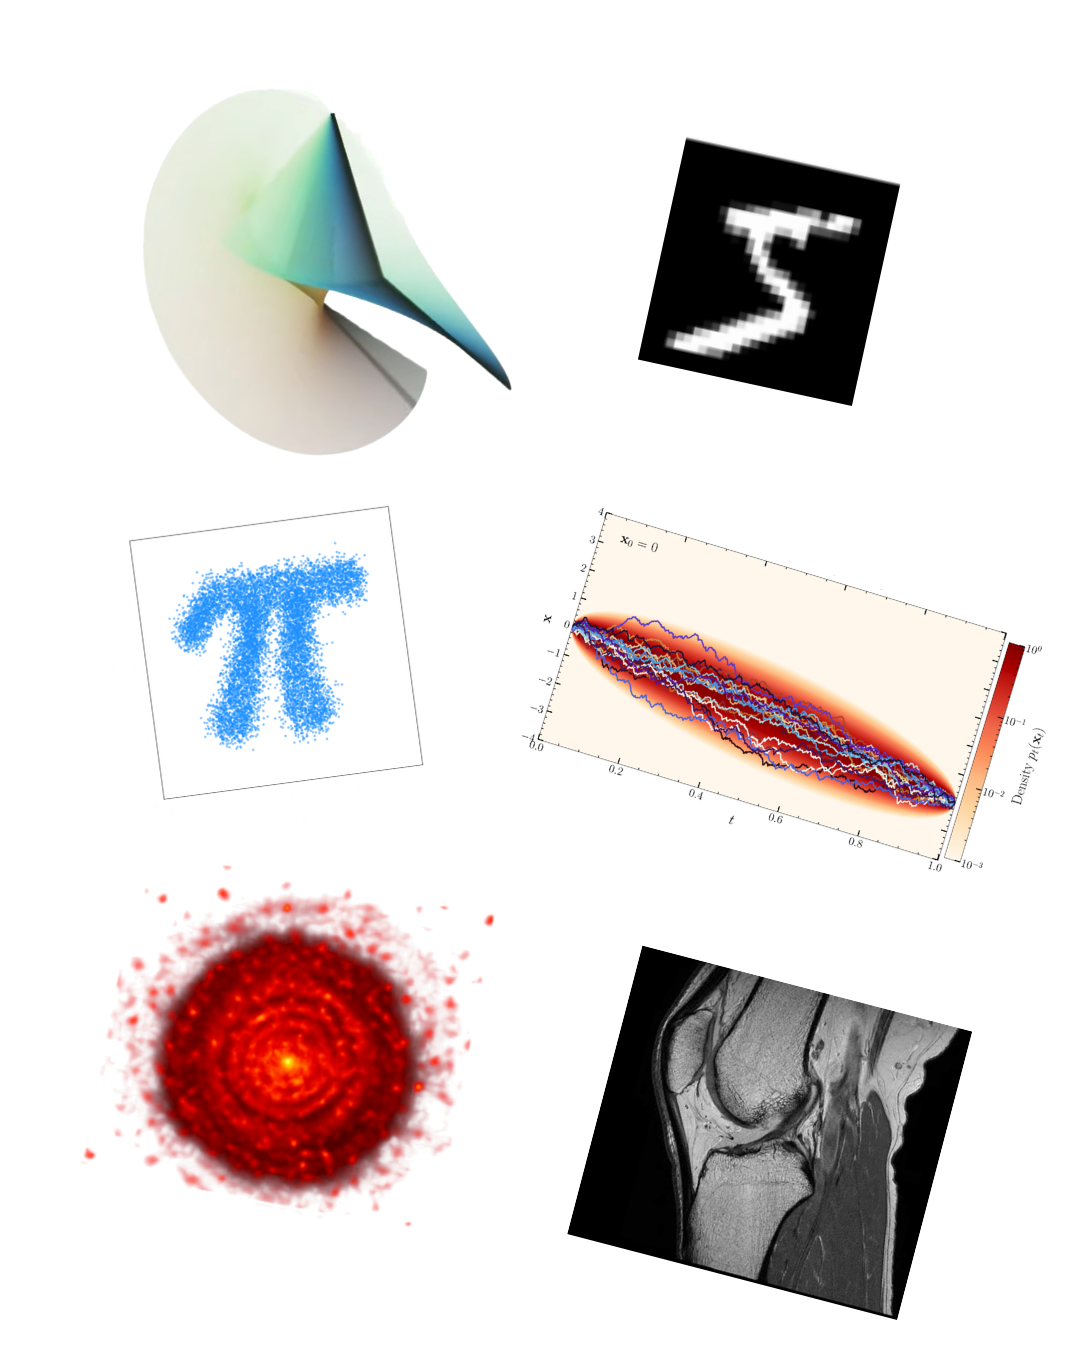
\includegraphics[scale=0.47]{figures/notes_cover.png}}
\date{}
\author{\Large Par Noé Dia. \\
}

% Renaming Reference section
\renewcommand{\bibsection}{\section*{Bibliography}}

\usepackage{titlesec}
% \defaultfontfeatures{Ligatures=TeX}
% \newfontfamily\subsubsectionfont[Color=MSLightBlue]{Times New Roman}
% Set formats for each heading level
\titleformat*{\section}{\Large\bfseries\sffamily\color{bordeaux}}
\titleformat*{\subsection}{\large\bfseries\sffamily\color{bordeaux!90}}
\titleformat*{\subsubsection}{\normalsize\bfseries\sffamily\color{bordeaux!80}}


\usepackage{mdframed}
\usepackage{framed}
\usepackage{xcolor}

\mdfdefinestyle{MyShadeQuoteStyle}{%
    leftmargin=15pt,
    rightmargin=15pt,
    backgroundcolor=dodgerblue!25,
    linewidth=0pt,
    skipbelow=\topskip,
    skipabove=\topskip
}

\newenvironment{shadequote}[1][]{%
    \ignorespaces%
    \begin{mdframed}[style=MyShadeQuoteStyle,#1]%
}{%
    \end{mdframed}%
    \ignorespacesafterend%
}%

\begin{document}

\maketitle
\fontsize{12}{14}\selectfont 
\vspace{-2cm}


\newpage
\tableofcontents
\newpage

\section{Notions de programmation en Python pour l'apprentissage profond.}\label{sec:programming}
\subsection{Pourquoi Python ?}
Python est un langage de programmation qui a été créé en 1991 par un informaticien néerlandais nommé Guido van Rossum. Ce qui caractérise ce langage de programmation c'est la grande liberté qu'il offre pour créer des programmes algorithmiquement complexes tout en gardant une syntaxe simple à lire et à comprendre. Comme le dit le créateur de Python,

\begin{shadequote}
    Python est une expérience afin de savoir la quantité de liberté dont un programmeur a besoin. Trop de liberté et personne ne peut lire le code de quelqu'un d'autre. Pas assez et l'expressivité est mise en danger. \textit{Guido van Rossum}
\end{shadequote}

Python est open-source, ce qui veut dire que le code source du langage de programmation est accessible à tous. De par sa flexibilité, sa simplicité, et son caractère open-source Python est un langage de programmation de choix pour les scientifiques. De la modélisation du climat à l'imagerie de trous noirs, Python est utilisée dans beaucoup de domaines scientifiques --- astrophysique, médecine, bio-informatique, climatologie, hydrodynamique etc...  Finalement, Python est également le langage de programmation à connaître pour pouvoir faire de l'apprentissage machine et de l'apprentissage profond (ou de l'intelligence artificielle si vous préférez ce terme).    

Vous l'aurez compris, si vous êtes intéressés par les sciences, connaître un langage de programmation est un gros atout à ajouter à votre CV. L'objectif de ce premier chapitre est donc de vous faire développer des compétences de programmation en Python. À l'issue de ce chapitre, vous devriez avoir les compétences nécessaires pour réaliser les mini-projets de modélisation numérique de système physique \Cref{sec:mini_projects}. Cela vous donnera également les bases nécessaires pour la programmation de réseaux de neurones que nous verrons \Cref{sec:ai}. 

\subsection{Notation}\label{subsec_1.1:notation}
En terme de notation, les variables de programmation seront écrites en monospace, c'est-à-dire, \texttt{comme ça}. J'utiliserai parfois ce qu'on appelle du pseudo-code, c'est-à-dire une version simplifiée d'un programme. Voir l'exemple ci-dessous.

\begin{algorithm}
$i\gets 10$\;
\eIf{$i\geq 5$}
{
    $i\gets i-1$\;
}{
    \If{$i\leq 3$}
    {
        $i\gets i+2$\;
    }
}
\end{algorithm}

\noindent Finalement, le code normal sera montré comme ci-dessous. 
\begin{minted}{python}
import torch
from torch import nn


class Simple_MLP(nn.Module):
    def __init__(
        self, 
        input_dim = int(28 * 28), 
        hidden_dim = 512, 
        output_dim = 10
        ):
        super().__init__()
        self.flatten = nn.Flatten()
        self.net = nn.Sequential(
            nn.Linear(input_dim, hidden_dim),
            nn.LeakyReLU(),
            nn.Linear(hidden_dim, hidden_dim),
            nn.LeakyReLU(),
            nn.Linear(hidden_dim, output_dim),
        )

    def forward(self, x):
        x = self.flatten(x)
        logits = self.net(x)
        return logits
\end{minted}
% \caption{Exemple code}

\subsection{Installer Python}
\subsubsection{Google Colab (recommandé sur l'ordinateur du laboratoire)}
Google Colab permet de créer des programmes en Python interactifs (ce qu'on appelle des \textit{notebooks}) sur une machine à distance. Cela va être très utile pour nous une fois qu'on voudra utiliser des machines plus performantes pour entraîner nos modèles en utilisant l'apprentissage automatique.
\begin{center}
\textbf{\textit{Si vous n'avez pas d'ordinateur portable et que vous utilisez l'ordinateur du laboratoire, je vous invite à utiliser Google Colab.}}
\end{center}
\subsubsection{Installer Python et utiliser VS code (recommandé sur votre ordinateur personnel)}

La seconde option est d'installer une version de Python et d'utiliser un éditeur de code. On va utiliser la version 3.11 de Python pour s'assurer de tous avoir la même version. Voici les étapes à suivre:
\begin{itemize}
    \item Allez sur le site officiel de python à la page de la version 3.11 en suivant \href{https://www.python.org/downloads/release/python-3119/}{ce lien}.
    \item Scrollez en bas de la page et cliquez sur le bouton d'installation qui correspond à votre système d'exploitation (soit Mac soit Windows). 
\end{itemize}


Dans le cadre de ce cours, je vous invite à utiliser VS Code comme éditeur de code. VS Code est un éditeur de code très populaire et pratique aussi bien pour les professionnels que pour les néophytes. Spécifiquement, on parle d'Environnement de Développement Intégré (en anglais \textit{Integrated Development Environment} ou IDE) lorsqu'on parle de logiciels tels que VS Code, PyCharm etc... Voici certains avantages forts qui font de VS Code un IDE particulièrement attractif:

\begin{itemize}[label=\raisebox{-1pt}{\scalebox{1.5}{\twemoji{heartpulse}}}]
    \item VS Code ne se limite pas à un seul langage. C'est un éditeur de code avec lequel on peut travailler pour la majorité des langages de programmations. Que ce soit du C++, du Fortran, du Python, du R etc... Donc, ça permet d'avoir dans un seul logiciel plein de possibilités de programmation. 
    \item C'est gratuit. On peut pas faire plus cher que gratuit. Donc, c'est plutôt pratique.
    \item Il y a beaucoup de possibilités de personnalisation pour une expérience de programmation agréable au quotidien. 
\end{itemize}

Vous comprendrez que cette sous-section est biaisée parce que je suis un fan de VS Code. Je n'ai jamais testé d'autres IDE que celui-là. Cependant, comme vous êtes jeunes, vous avez le droit d'être rebels et si vous voulez tester autre chose, allez-y :). 
C'est à vos risques et périls ...

\subsubsection{Environnement virtuel}
Si vous choisissez l'option VS Code, je vous conseille de créer un environnement virtuel. Lorsqu'on démarre un projet, il est conseillé de créer un environnement virtuel qui regroupera tous les packages nécessaires pour le fonctionnement du projet. C'est très important de faire ceci, sinon on se retrouve avec plusieurs projets qui nécessitent différentes versions d'un package en particulier et ça peut devenir très chaotique (oui, ça m'est déjà arrivé... c'est l'expérience qui parle...). Vous pouvez considérer ce cours comme un projet qui nécessitera exactement un environnement virtuel. 

Une fois votre fenêtre VS Code ouverte, faîtes la commande Ctrl+Shift+P. Ceci devrait ouvrir une fenêtre de recherche dans laquelle vous pouvez taper "Environnement". Il devrait ensuite s'afficher dans la barre de recherche une option "Python: Create environment..." (ou la même chose mais en français) comme montré Figure \ref{fig:vscode-screenshot}. Cliquez sur cette option. 
Cliquez ensuite sur l'option venv. Une fenêtre va s'ouvrir pour choisir quelle version de Python à utiliser. Si Python est bien installé, la version 3.11 devrait apparaître. Choisissez cette version. 

Sur Windows, vous pouvez activer l'environnement virtuel, en ouvrant le terminal de commande (Ctrl+`) et en tappant ".venv/Scripts/activate/". Si vous êtes sur Mac ou Linux, vous devez taper ".venv/bin/activate".
Une fois l'environnement virtuel activé, installez quelques librairies dont on aura besoin pendant le cours avec la commande 
\texttt{pip install numpy matplotlib ipykernel torch torchvision} que vous écrirez dans le terminal de commande.
\begin{figure}
    \centering
    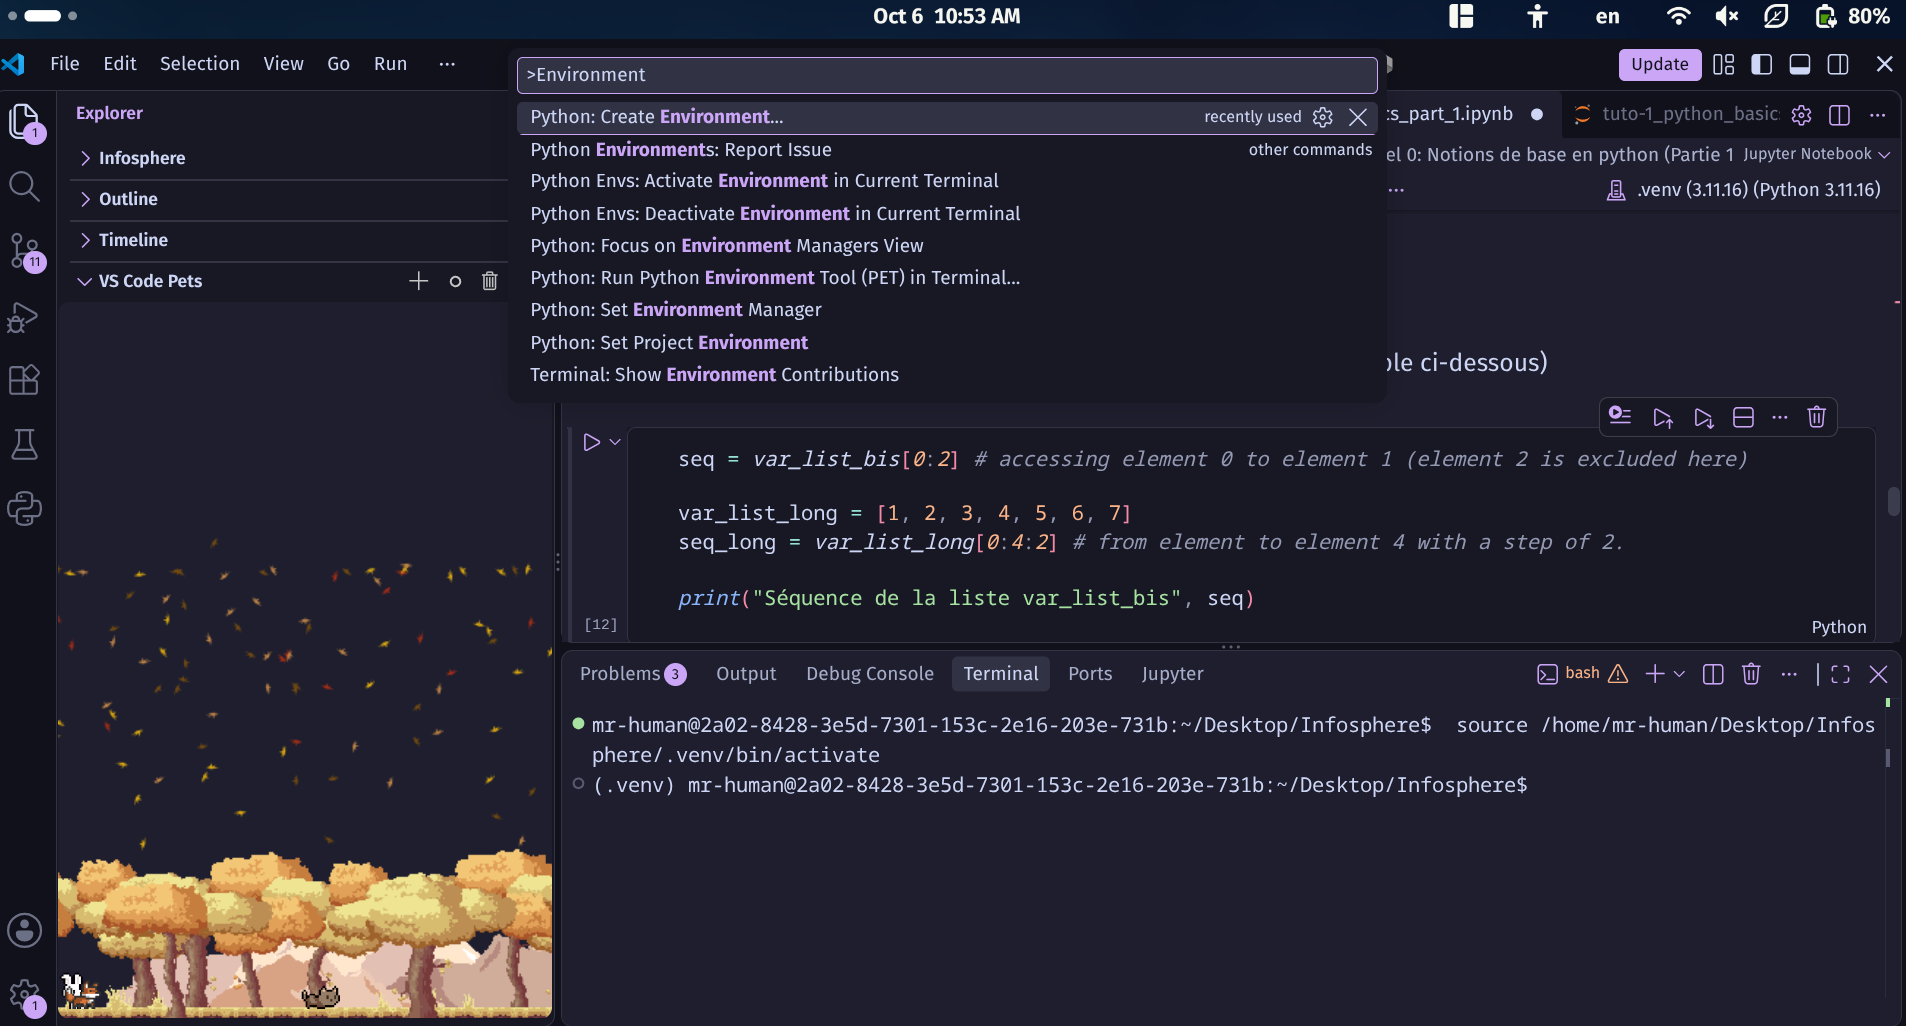
\includegraphics[scale=0.2]{figures/Screenshot From 2026-10-06 10-53-29.png}
    \caption{Créer un environnement virtuel sur VS Code}
    \label{fig:vscode-screenshot}
\end{figure}

\subsubsection{(Optionnel) Plugins}
Vous pouvez installer des plugins pour rendre votre VS Code plus joli.
En voici quelques uns


\subsection{Notions de base en Python}

\subsubsection{Les différents types variables et d'opérations en Python}
Il existe plusieurs types de variables en Python, 
\begin{itemize}
    \item Les variables contenant un nombre entier de type \texttt{int} (\textit{integer} à voix haute)  
    \item Les variables contenant un nombre réel de type \texttt{float}.
    \item Les variables contenant du texte. Elles sont de type \texttt{str} (\textit{string} à voix haute).
    \item Les variables contenant une séquence dynamique d'éléments. Ces variables sont de type \texttt{list}. 
    \item Les variables contenant une séquence statique d'éléments. Ces variables sont de type \texttt{tuple}\footnote{La traduction française du mot "tuple" est $n$-uplet selon la documentation officielle de Python. J'utiliserai néanmoins l'anglicisme "tuple" dans le reste des notes de cours.}.
    \item Les variables fonctionnant comme un dictionnaire où à une variable de type \texttt{str} est associée une valeur. Ces variables sont de type \texttt{dict}.
    \item Les variables qui sont soit \texttt{True}, soit \texttt{False}. Ces variables sont de type \texttt{bool} et sont dites \textit{booléennes}.
\end{itemize}

En Python, une variable est instantiée via l'opérateur \texttt{=} qui est \textit{un opérateur d'affectation}. Un résumé des différentes variables est donnée \Cref{tab:python_variables} avec un exemple d'instantiation pour chaque type de variable (pour que vous connaissiez la syntaxe associée à chaque type).

\begin{table}[h!]
    \centering
    \begin{tabular}{c|c}
         Exemple de Variable & Type  \\
        \hline 
        \hline
        \texttt{x = 3}       & \texttt{int}\\
        \texttt{x = 42.24}       & \texttt{float}\\
        \texttt{x = "Hey"}       & \texttt{str}\\
        \texttt{x = ["banana", "apple", "strawberry"]}       & \texttt{list}\\
        \texttt{x = ("peas", "beans", "spinach")}       & \texttt{tuple}\\
        \texttt{x=\{"sky": "blue", "grass": "green"\}}       & \texttt{dict}\\
        \texttt{x = True}       & \texttt{bool}
    \end{tabular}
    \caption{Exemple de variable et leur type associé.}
    \label{tab:python_variables}
\end{table}

Il existe également plusieurs opérations, et donc plusieurs opérateurs en Python. On compte, 
\begin{enumerate}
    \item les opérateurs arithmétiques: addition, soustraction, division, puissance, modulo (reste d'une division euclidienne), division entière (quotient d'une division euclidienne)
    \item les opérateurs logiques: \texttt{and}, \texttt{or} et \texttt{not}. Ils sont utilisés pour des opérations entre variables booléennes.
    \item les opérateurs relationnels ou de comparaison: ils permettent de tester des inégalités mathématiques (opérateurs \texttt{>}, \texttt{<}, \texttt{<=}, \texttt{>=}), des égalités (opérateur \texttt{==}), des différences (opérateur \texttt{!=}) ou l'appartenance dans le cas des variables contenant des séquences (opérateur \texttt{in}). Des exemples d'utilisation de ces opérateurs vous sont joints \Cref{tab:ops_comparison}. 
\end{enumerate}


\begin{table}[h!]
    \centering
    \begin{tabular}{c|c|c}
         Opérateur relationnel & Exemple d'utilisation & Signification\\
        \hline 
        \hline
        \texttt{>}       & \texttt{a > b} & Teste si $a>b$. Retourne \texttt{True} si c'est le cas. \\
        \texttt{<}       & \texttt{a < b} & Teste si $a<b$. Retourne \texttt{True} si c'est le cas. \\
        \texttt{>=}       & \texttt{a >= b} & Teste si $a\geq b$. Retourne \texttt{True} si c'est le cas. \\
        \texttt{<=}       & \texttt{a <= b} & Teste si $a\leq b$. Retourne \texttt{True} si c'est le cas. \\
        \texttt{==}       &  \texttt{a == b} & Teste si $a=b$. Retourne \texttt{True} si c'est le cas. \\
        \texttt{!=}       & \texttt{a != b} & Teste si $a\neq b$. Retourne \texttt{True} si c'est le cas.\\
        \texttt{in}       & \texttt{a in b} & Teste si $a$ est contenue  dans la séquence $b$. 
    \end{tabular}
    \caption{Exemple d'utilisation des opérateurs relationnels (ou de comparaison).}
    \label{tab:ops_comparison}
\end{table}

Les opérateurs arithmétiques ont des comportements spécifiques lorsqu'utilisé sur des variables correspondant à des chaînes de caractères, ou des séquences (liste et tuple par exemple). 

\subsubsection{Les instructions \texttt{if}, \texttt{elif} et \texttt{else}}
En programmation, il sera parfois utile d'exécuter différents de blocs selon si une condition est satisfaite ou non. Les instructions \texttt{if} (qui se traduit "si"), \texttt{elif} (qui est le diminutif de "else if" en anglais se traduisant "ou si") et \texttt{else} (qui se traduit "sinon"). 

Un bon exemple tiré de la physique est celui des transitions de phase. Par exemple, l'eau va changer d'état à partir de certaines températures critiques. En dessous de 0 degrés Celsius, on a de la glace, l'eau est à l'état solide. Lorsque la température dépasse les 100 degrés Celsius, l'eau passe sous forme gazeuse. Finalement, entre ces deux températures critiques, 
l'eau est à l'état liquide. On pourrait donc écrire un code comme celui-ci dessous pour changer les instructions à exécuter selon l'état dans lequel l'eau est.


\begin{minted}{python}
    temperature = ... # to fill

    if temperature > 100:
        water_state = "gas"
        # do something 1
    elif temperature < 0:
        water_state = "solid"
        # do something 2
    else:
        water_state = "liquid"
        # do something 3
\end{minted}

On peut ajouter autant de contraintes nécessaires si on 
ajoute simplement des \texttt{elif} dans la même structure que ci-dessus. 

\subsubsection{Les boucles \texttt{for} et \texttt{while}}
Les boucles vont être utiles pour faire des itérations. Les itérations peuvent intervenir 
lors du calcul d'une série qui approxime $\pi$, lors de la résolution d'un système physique comme le double pendule,
lors de la recherche des zéros d'une fonction ou de ces extrema etc... En bref, il est difficile de se 
passer des boucles et de l'itération quand on fait de la programmation.



La boucle \texttt{for} est une boucle dite inconditionnelle. Elle permet d'itérer 
sur les éléments de séquences comme les variables de type \texttt{list}, \texttt{tuple}, \texttt{dict}.
Pour itérer sur des suites arithmétiques, la boucle \texttt{for} peut être utilisé en conjonction
avec la fonction \texttt{range} qui crée une séquence de nombres. Par exemple,
\begin{minted}{python3}
    a = list(range(5))
\end{minted}
va assigner à la variable \texttt{a} la liste \texttt{[0, 1, 2, 3, 4]} soit une séquence d'entiers qui va de 0 à 5 exclu avec un pas de 1.
Il est possible de contrôler la taille du pas qui est fait par la fonction et l'entier à partir duquel la séquence commence comme suit
\begin{minted}{python3}
    a = list(range(1, 10, 2))
\end{minted}
ce qui assigne à la variable \texttt{a} la liste \texttt{[1, 3, 5, 7, 9]}. 
On peut ensuite utiliser la fonction \texttt{range} avec la boucle \texttt{for} comme suit
\begin{minted}{python}
    s = 0
    for i in range(5):
        s += i
\end{minted}
Le code ci-dessus calcule la somme suivante
\begin{equation*}
    S = 1+2+3+4
\end{equation*}
En notation mathématique formelle, on utilisera le symbole $\Sigma$ pour noter la somme
\begin{equation*}
S = \sum_{i=1}^ {4} i
\end{equation*}


\begin{example}{Formule de Madhava-Leibniz de $\pi$}{}
   La formule de Madhava-Leibniz permet de trouver une expression de $\pi$ sous la forme 
   d'une série alternée,
   \begin{equation*}
   \frac{\pi}{4} = \sum_{i=0}^{\infty}\frac{(-1)^{i}}{2i + 1}
   \end{equation*}

   On peut calculer les $N$ premiers termes de la série en utilisant une boucle \texttt{for} avec le code suivant
   \begin{minted}{python3}
    s = 0
    N = 200
    for i in range(N)
        s += (-1) ** (i) / (2 * i + 1)
   \end{minted}
   ce qui est équivalent à évaluer 
   \begin{equation*}
   \frac{\pi}{4} = \sum_{i=0}^{200}\frac{(-1)^{i}}{2i + 1}
   \end{equation*}
   Bien entendu, plus on augmente $N$, plus on a une meilleure approximation de $\pi$ mais plus il faut de temps pour l'ordinateur pour calculer les termes de la somme.
\end{example}

\begin{example}{Double somme}{}
    Vous l'aurez peut-être deviné mais pour calculer une double somme, il suffira de faire appel deux fois à une boucle \texttt{for}.
    Par exemple, cette double somme
    \begin{align}
        S = \sum_{i=1}^{M} \sum_{j=1}^{N} i+j \, ,
    \end{align}
    peut être calculée avec le code suivant
    \begin{minted}{python}
    s = 0
        for i in range(1, M+1):
            for j in range(1, N+1):
                s+= i + j
    \end{minted}
\end{example}

\subsubsection{Les fonctions et les méthodes}

\subsubsection{Les erreurs}
Différents types d'erreurs en python. 

\subsubsection{La programmation orientée objet}

\subsubsection{Données tabulées et figures avec \texttt{numpy} et \texttt{matplotlib}}

\begin{itemize}
    \item Montrer comment faire des opérations avec données tabulées
    \item Montrer comment sauvegarder des données numpy dans des fichier \texttt{.npy} ou \texttt{.npz}. 
    \item Montrer comment 
    \item Montrer comment faire une figure pour une image. 
    \item Montrer comment faire une figure pour des points de données (courbes)
    \item Montrer comment faire une figure en remplissant une zone avec un alpha pour la transparence. 
\end{itemize}

Expliquer l'importance de checker la documentation. 

\subsection{PyTorch: Le package pour faire de l'apprentissage profond.}

\section{Notions mathématiques pour l'apprentissage profond.}

\subsection{Algèbre linéaire et calcul matriciel}
\subsubsection{Opérations matricielles}

\subsubsection{Trace d'une matrice}

\subsubsection{Déterminant d'une matrice}

\subsubsection{Résolution d'un système d'équations linéaire}

Algorithme de Gauss-Jordan.


\subsection{Calcul à plusieurs variables}
\subsubsection{La dérivée en 3D et hautes dimensions: l'opérateur gradient}
exemple de calcul du gradient d'une fonction à 2 variables. Exemple de trouver points de selle, maxima et minima. 

\subsubsection{L'intégrale en 3D et hautes dimensions}


Changement de variables dans l'intégrale avec Jacobien. 

\subsubsection{Équations différentielles.}

\subsection{Théorie des Probabilités et Statistiques}
\subsubsection{Fréquentisme ou Bayésianisme, telle est la question...}
Afin de parler statistiques, nous devons inévitablement définir clairement la notion de \textit{probabilité}. 
Il existe deux définitions associées à deux écoles de pensée: le fréquentisme et le bayésianisme. 

Dans la vision fréquentiste, une probabilité est définie comme la fréquence à long-terme d'événements qui peuvent se produire plusieurs fois. C'est la définition des probabilités que vous avez apprise au lycée en seconde ou en première. En gros, adopter cette vision, c'est dire: "Si je répète une  expérience aléatoire $N$ fois avec $N$ qui tend vers l'infini ($N\rightarrow\infty$), combien de fois j'obtiendrai l'événement $X$".

La seconde perspective (ma préférée) est la vision bayésienne des probabilités. Dans cette vision, la probabilité est définie pour déterminer notre incertitude, notre ignorance sur quelque chose. 
Prenons un exemple. Disons que je veux connaître mon incertitude sur la météo qu'il y aura demain le 26/09 

\subsubsection{Expériences aléatoires et définition des probabilités}

\begin{definition}{Expérience aléatoire, événement}{}
    La notion de probabilité va survenir lorsqu'on considérera une expérience aléatoire.
    
    \textit{\textbf{Une expérience aléatoire} est une expérience dont les résultats possibles sont connus mais dont le résultat final est dû au hasard.}
    
    \textit{\textbf{Un événement} correspond à un des différents résultats possibles à l'issue d'une expérience aléatoire.} 


On peut voir une probabilité comme une fonction qui va prendre en entrée un événement $X$ et qui va donner en sortie un nombre réel entre 0 et 1 qui correspond à la possibilité que l`événement $X$ se réalise. Plus le nombre est proche de 1 plus il y a de chances que l'événement se réalise. L'événement a donc une probabilité élevée de se réaliser. Lorsque le nombre est proche de 0, l'événement a une probabilité faible de se produire.
\end{definition}

\begin{example}{Expérience aléatoire et événement}{}
    On rencontre des expériences aléatoires absolument partout dans notre quotidien sans vraiment s'en rendre compte.
    Certaines expériences aléatoires font intervenir des probabilités dites discrètes: le jet d'un dé, le lancer d'une pièce... 
    D'autres font intervenir des probabilités dites continues. Elles permettent aussi de poser des questions telles que: (i) quelle est la probabilité que la durée de vie d'un smartphone soit inférieure à deux ans ? (ii) quelle est la probabilité que mon sachet de pâtes fasse (200 $\pm$ 10)g ? (iii) quelle est la probabilité que deux élèves d'une classe de 30 aient la même date d'anniversaire ?
    (iv) quelle est la probabilité qu'une exoplanète ait été détectée par le James Webb Space Telescope ? 

    Lorsqu'une expérience aléatoire font intervenir une loi de probabilité connue, on dit que l'expérience aléatoire \textit{suit} la loi de probabilité. Par exemple, le lancer d'un dé suit une loi uniforme.
\end{example}
Exemple: La fonction $f(x)=x^2$ prend en entrée une valeur de $x\in \mathbb{R}$ et donne en sortie une valeur $y=x^2$ où $y\in \mathbb{R}$. 

On va faire la distinction entre deux types de probabilité,
\begin{itemize}
    \item Les probabilités discrètes, celles qu`on utilise pour décrire des expériences aléatoires telles qu'un lancer de dé, un lancer de pièce, jouer à pierre-feuille-ciseaux...
    \item les probabilités continues celles qu'on utilise pour estimer la probabilité que la durée de vie d'un smartphone soit inférieure à 2 ans, ou encore la probabilité qu'une intelligence artificielle nous annihile tous entre 2026 et 2036 etc...
\end{itemize}  et . 




\subsubsection{Probabilités discrètes}
Dans le cadre des probabilités discrètes, on va considérer une \textit{expérience aléatoire}, c'est-à-dire une expérience dont les résultats possibles sont connus mais dont le résultat final est dû au hasard. Un exemple que vous avez sûrement étudié par le passé est le jet d'un dé. 
Il existe 6 résultats possibles lors d'un jet de dés mais une fois que le dé est lancé, dur de savoir quelle face du dé nous fera face ;).
On appellera \textit{événement} les différents résultats possibles de l'expérience aléatoire. L'ensemble des événements sera noté $\Omega$, aussi appelé \textit{espace d'échantillonnage} (``sample space" en anglais). Dans le cadre de notre lancer de dé, l'espace d'échantillonage peut être écrit,
\begin{align}
    \Omega &= \{A, B, C, D, E, F\},
\end{align}
et les différents événements $A,B,C,D,E,F$ correspondent aux résultats possibles suivants, 
\begin{align}
    A &= \text{Obtenir la face ``1"} \, ,
    \\
    B &= \text{Obtenir la face ``2"}\, ,
    \\
    C &= \text{Obtenir la face ``3"}\, ,
    \\
    D &= \text{Obtenir la face ``4"}\, ,
    \\
    E &= \text{Obtenir la face ``5"}\, ,
    \\
    F &= \text{Obtenir la face ``6"}\, .
\end{align}

Pour les probabilités discrètes, on notera $P(\cdot)$ la fonction qui prend en entrée un événement $X$ et qui donne en sortie la probabilité que cet événement se produise. Cette fonction est nommée la \textit{fonction de probabilité de masse}\footnote{Ce nom provient de la physique où l'on appelle masse les objets ponctuels sans volume et où l'on va parler de densité lorsqu'un objet avec une forme, un volume occupe un espace. On verra que, lorsqu'on parle de probabilités continues, l'équivalent de la fonction de probabilité de masse est la fonction de probabilité de densité.}. 

Pour notre jet de dé, on a
\begin{equation}
    P(A)=P(B)=\dots = P(F) = \frac{1}{6}
\end{equation}

On peut visualiser ça graphiquement Figure ...

Lorsque tous les événements de l'espace d'échantillonnage ont la même probabilité, on dit alors que l'expérience aléatoire suit une \textit{loi de probabilité uniforme} ou simplement \textit{loi uniforme}. Lorsqu'une pmf est constante pour tout événement, on notera
\begin{align}
    P(X)=\mathcal{U}(X)\, .
\end{align}
où $\mathcal{U}(X)$ est une fonction constante, i.e.
\begin{align}
    \mathcal{U}(X)=\frac{1}{\lvert \Omega \rvert}=\text{cste} \quad \forall X\in \Omega
\end{align}
où $\lvert \Omega\rvert$ dénote la cardinalité de l'espace d'échantillonnage $\Omega$. La cardinalité correspond au nombre d'éléments composant l'ensemble $\Omega$. Dans notre exemple du lancer de dé, on dit que l'espace d'échantillonnage est fini\footnote{tout simplement parce qu'on peut compter le nombre d'éléments de l'espace d'échantillonnage} et qu'il a une cardinalité égale à 6, i.e. $\lvert \Omega \rvert = 6$. 

\subsubsection{Moyenne et déviation standard d'une distribution de probabilité discrète}
Pour des distributions de probabilité (discrètes ou continues), il sera intéressant d'étudier la moyenne et la déviation standard d'une distribution de probabilité.

Admettons une expérience aléatoire qui a été faite un nombre $N$ de fois. Disons par exemple qu'on a lancé $N$ fois un dé. On veut maintenant savoir sur quelle face le dé tombe en moyenne.  

\begin{definition}{Moyenne et écart-type d'une distribution de probabilité discrète}{prob_discrete}
    La formule générale pour calculer la moyenne d'une probabilité discrète est donnée par,
    \begin{align}
        \mu(X)=\mathbb{E}(X) \equiv \frac{1}{N}\sum_{i=1}^{N}x_iP(X=x_i) \, .
    \end{align}
    où $X\in \Omega =\{x_1, x_2,x_3,x_4,x_5, x_6 \}= \{1,2,3,4,5,6\}$.
    
    La moyenne n'est pas à confondre avec la médiane ou encore le mode d'une distribution de probabilité. La médiane est le point milieu d'une séquence de données telle que 50\% des données ont une valeur inférieure et 50\% ont une valeur supérieure. 

    La formule générale pour calculer l'écart-type d'une probabilité discrète est définie à partir de la moyenne comme, 
    \begin{align}
        \sigma(X) \equiv \sqrt{\text{Var}(X)}&=\sqrt{\mathbb{E}[(X-\mathbb{E}[X])^2]}
        \\
        &=\sqrt{\mathbb{E}[X^2]-\mathbb{E}[X]^2}
        \\
        &=\sqrt{\frac{1}{N}\sum_{i=1}^{N}P(X=x_i)(x_i-\mu)^2}
    \end{align}
    La déviation standard va être une mesure de la dispersion de la distribution de probabilité (à quel point elle s'étale).
\end{definition}


\begin{example}{Moyenne et déviation standard pour 10 lancers de dé}{}
    
\end{example}




\subsubsection{Exemples de lois de probabilité discrètes}
Uniforme
Binomial


\subsection{Probabilités continues.}
On peut également assigner une densité de probabilité à des vecteurs. Par exemple, si je note, 
$p(\mathbf{x})$


Notez qu'on peut unifier les probabilités discrètes et les probabilités continues avec la \textit{théorie de la mesure}. Vous verrez ceci dans vos études supérieures si vous continuez sur ce chemin-là en mathématiques et/ou en intelligence artificielle. On pourra en discuter brièvement si certain(e)s d'entre vous sont vraiment intéressé(e)s.    


\subsubsection{Probabilités jointes, conditionnelles et théorème de Bayes}

\subsubsection{Quelques distributions de probabilité communes...}


\subsection{Introduction à la théorie de l'Information}



\section{Intelligence Artificielle, Apprentissage Machine et Apprentissage Profond}\label{sec:ai}


\subsection{Histoire et définitions...}
Mouvements philosophiques associés à l'IA 
Cybernétiques etc...

\subsection{Fondements de l'apprentissage machine}

\subsubsection{Théoreme d'approximation universelle ou Théoreme de Cybenko: le pilier fondateur de l'apprentissage profond}

\subsubsection{Réseaux de neurones comme machines à apprendre des fonctions}

\subsubsection{Entrainement de réseaux de neurones: maximisation de la vraisemblance.}
Fonction d'erreur définition comme negative log likelihood. 

\subsubsection{Régularisation et Hyperparameter tuning pour éviter le sur-ajustement et le sous-ajustement}

Régularisation = prior on the weights


Yoshua Bengio. 


Créateur des Gans
Créateur des VAEs
Créateur des Diffusion models. 

Katie Bouman, Berthy Feng. 

\subsection{Classificateur}

\subsection{Inférence basée sur des simulations}

\subsection{Modèles génératifs}


\section{Mini-projets de programmation}\label{sec:mini_projects}
\subsection{Simulation d'un double pendule}
On cherche à simuler un double pendule en utilisant le package \texttt{scipy} qui va nous permettre de résoudre un système d'équations différentielles de la forme
\begin{align}
    \omega_1 &= \frac{d\theta_1}{dt}
    \\
    \omega_2&= \frac{d\theta_2}{dt}
    \\
    \frac{d\omega_1}{dt} &=\frac{d^2\theta_1}{dt^2} = \dots
    \\
    \frac{d \omega_2}{dt}&=\frac{d^2\theta_2}{dt^2}=\dots
\end{align}
Ici, il nous reste à trouver les expressions des dernières équations. Comme je suis gentil, je vous les donne. Pour ceux qui sont intéressés, je vous donne la dérivation complète en annexe.


Voici le système d'équations complets que vous devez simuler:
\begin{align}
    \begin{pmatrix}
        \omega_1 \\
        \omega_2 \\
        \dot{\omega_1} \\
        \dot{\omega_2}
    \end{pmatrix}
    &=
\end{align}

\subsection{Étude des courbes de Lissajous}
Voir notes cours wolfram

\subsection{Simulation d'un spirographe, hypotrochoïdes et cie.}
Voir lab de physique numérique

\subsection{Étude du chaos avec les attracteurs}
Les attracteurs sont des modèles mathématiques qui interviennent lors de l
(voir notes de cours Paul Charbonneau)

\subsection{Le problème à trois corps.}

\section{Projets d'apprentissage automatique et programmation}
\subsection{Inférence bayésienne d'images avec modèles de diffusion en radio interférométrie et IRM}


\subsection{Inférence bayésienne d'images avec normalizing flows}


\subsection{Transport optimal avec interpolant stochastique.}

\subsection{Apprentissage de distribution a priori sur Lénia}









\newpage
\bibliographystyle{apalike}
\bibliography{references}

\appendix 

\section{Matériel supplémentaire pour les exercices de physique}
Cette section contient des dérivations mises au propre pour certains exercices
de physique que vous avez pu voir dans les exercices de programmation que je vous 
ai donnés. 

\subsection{Le lanceur de poids}
Dans cette sous-section, je vous présente la dérivation complète (i) pour calculer
une expression pour le vecteur position $\vec{r}(t)=(x(t), y(t))$, (ii) calculer le temps de vol du poids
(iii) calculer la portée, soit la distance en $x$ parcourue par le poids. J'ai choisi la discipline du lancer de poids
ici, dont je présente les détenteurs des record du monde masculin et féminin \Cref{fig:record_poids} mais la dérivation
est la même si on considère un lancer d'un objet quelconque dans un champ de gravitation uniforme.
\begin{figure}[h!]
    \begin{tikzpicture}
    \node (img1) at (0,0) {
    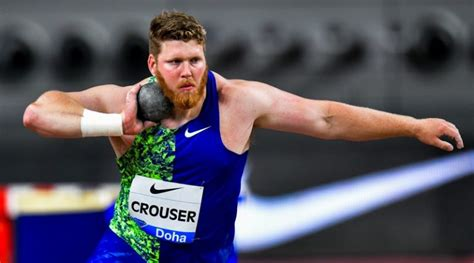
\includegraphics[scale=0.5]{figures/image.jpeg}
    };
    \node (img2) at ([xshift=0.5cm]img1.east) [anchor=west] {
    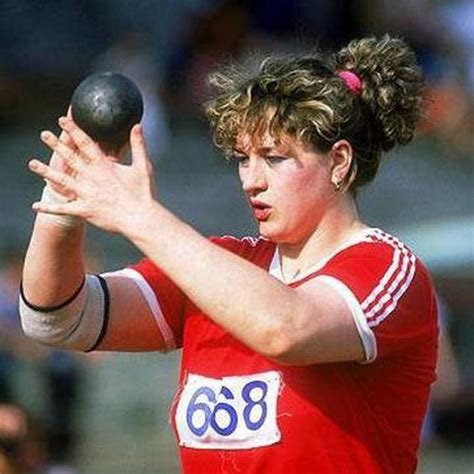
\includegraphics[scale=0.3]{figures/image_woman.jpg}
    };
\end{tikzpicture}
\caption{Ryan Crouser et Natalya Lisovskaya, détenteurs du record du monde de lancer de poids dans leurs catégories respectives (23,56 m et 22,63 m).}
\label{fig:record_poids}
\end{figure}


\subsubsection{Équations horaires}
Commençons par la dérivation des équations horaires du poids. La première étape est de faire un bilan des forces que subit le poids.
Dans notre cas, on va ignorer la résistance de l'air et assumer que seule la force gravitationnelle agit sur le poids,
\begin{equation}
    \vec{F} = -mg \hat{\mathbf{y}}\, ,
\end{equation}
où $\hat{\mathbf{y}}$ est le vecteur directeur de l'axe des ordonnées qui pointe directement vers le haut.

De plus, on va assumer connaître la vitesse initiale $v_0$ à laquelle le poids est lancé et l'angle $\theta$ que fait le poids avec
l'horizontale. Ceci veut dire qu'à $t=0$, le vecteur vitesse est connu et a la forme suivante,
\begin{equation}\label{eq:init_conds_poids}
    \vec{v}(t)\Longrightarrow
    \begin{cases}
        v_{x}(t=0) &= v_0\cos(\theta) \\
        v_{y}(t=0) &= v_0\sin(\theta)
    \end{cases}  \, .
\end{equation}

On connaît également la position initiale du poids à $t=0$, 
\begin{equation}\label{eq:init_conds_poids}
    \vec{r}(t) \Longrightarrow
    \begin{cases}
        x(t=0) &= x_0 \\
        y(t=0) &= y_0
    \end{cases}  \, .
\end{equation}
Le bilan des forces et l'esquisse du système qu'on étudie vous sont présentés \Cref{fig:lanceur_poids}.
\begin{figure}[h!]
    \centering
    \begin{tikzpicture}
    \node (img1) at (0,0) {
    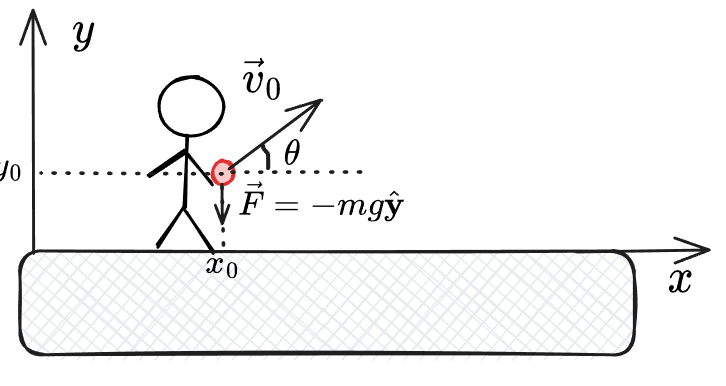
\includegraphics[scale=0.4]{figures/lanceur_poids.png}
    };
\end{tikzpicture}
\vspace{-0.5cm}
\caption{Bilan des forces sur le poids. La résistance de l'air est assumée négligeable.}
\label{fig:lanceur_poids}
\end{figure}

Grâce au bilan des forces qu'on vient de faire, on obtient les équations de mouvement en appliquant la seconde loi de Newton, 
\begin{align}
    \sum \vec{F} = m \vec{a} \Longrightarrow  &\begin{cases}
    m a_x = 0 \\
    m a_y = - mg
    \end{cases}
    \\
    &\begin{cases}
        a_x = 0 \\
        a_y = -g
    \end{cases}\label{eq:motion_poids}
\end{align} 

On intègre maintenant par rapport au temps pour obtenir les équations du vecteur vitesse en fonction du temps. Rappelez-vous que, 
\begin{align}
    \vec{v}(t) -\vec{v}(t=0)&= \int_{0}^{t} \vec{a} dt'\, ,
    \\
    &= \int_{0}^{t} \frac{d\vec{v}}{dt'} dt'\, .
\end{align}
En isolant $\vec{v}(t)$, on a 
\begin{align}
    \vec{v}(t) = \vec{v}(t=0) + \int_{0}^{t} \vec{a} dt'
\end{align}
Allons-y maintenant composante par composante pour obtenir $v_x(t)$ et $v_y(t)$. Pour la composante en $x$, on a
\begin{align}
    v_x(t) &= v_x(t=0) + \int_{0}^{t} \underbrace{a_x}_{=0} dt'
    \\
    &= v_0\cos(\theta) 
\end{align}
où on a remplacé l'expression de $v_x(t=0)$ en utilisant \Cref{eq:init_conds_poids} et l'expression de $a_x$ en utilisant \Cref{eq:motion_poids}. 
On fait maintenant la même chose pour la composante $y$ de la vitesse, 
\begin{align}
    v_y(t) &= v_y(t=0) + \int_0^{t} \underbrace{a_y}_{=-g}dt'
    \\
    &= v_0\sin(\theta) + \int_0^{t}-g dt'
    \\
    &= v_0\sin(\theta) -g t
\end{align}

On réintègre une seconde fois par rapport au temps pour obtenir les équations horaires, soit le vecteur position en fonction du temps $\vec{r}(t)=(x(t), y(t))$. 
Rappelez-vous que, 
\begin{align}
    \vec{r}(t) - \vec{r}(t=0) &= \int_0^{t} \vec{v}dt' \\
    &= \int_0^{t} \frac{d \vec{r}}{dt'} dt'\, .
\end{align}
Par conséquent, 
\begin{align}
    \vec{r}(t) = \vec{r}(t=0) + \int_{0}^{t} \vec{v} dt' \, .
\end{align}
Résolvons maintenant l'intégrale composante par composante. Pour la composante $x$, on a
\begin{align}
    x(t) &= x(t=0) + \int_0^{t} v_x dt'\, ,
    \\
    &= x_0 + \int_{0}^{t} v_0\cos(\theta) dt'\, ,
    \\
    &= x_0 + v_0\cos(\theta) t\, ,
\end{align}
où on a remplacé la condition initiale $x(t=0)=x_0$ à la seconde ligne.

Pour la composante $y$, on a, 
\begin{align}
    y(t)&= y(t=0) + \int_0^{t} v_y dt' \, ,
    \\
    &= y_0 + \int_{0}^{t} v_0\sin(\theta) -gt' dt' \, ,
    \\
    &= y_0 + v_0\sin(\theta) t -\frac{1}{2}g t^2\, ,
\end{align}
où on a remplacé la condition initiale $y(t=0)=y_0$ à la seconde ligne. Pour récapituler, les équations horaires sont donc, 
\begin{align}\label{eq:horaires_poids}
    \tcbhighmath{\vec{r}(t)\Longrightarrow \begin{cases}
        x(t) &= v_0\cos(\theta) t + x_0
        \\
        y(t) &= -\frac{1}{2}gt^2 + v_0\sin(\theta) t + y_0
    \end{cases}}
\end{align}

\subsubsection{Équation de la trajectoire}
L'équation de la trajectoire est obtenue en exprimant $t$ en fonction de $x$ puis en remplaçant dans l'équation de $y(t)$.
De l' \Cref{eq:horaires_poids}, on a 
\begin{align}
    x - x_0 = v_0\cos(\theta)t \Longrightarrow t = \frac{x - x_0}{v_0\cos(\theta)}
\end{align}
On remplace maintenant dans $y(t)$ pour obtenir l'équation de la trajectoire, 
\begin{align}
    y(x) = -\frac{1}{2} g \left(\frac{x - x_0}{\cos(\theta)}\right)^2 +(x - x_0)\tan(\theta) + y_0
\end{align}
ce qui peut être réécrit comme,
\begin{align}
    y(x) = -\frac{1}{2}g \left(x-x_0\right)^2 \sec^2(\theta) + (x-x_0)\tan(\theta) + y_0
\end{align}
où $\sec(\theta)=\frac{1}{\cos(\theta)}$.

\subsubsection{Temps de vol}
Le temps de vol $T$ est obtenu en résolvant l'équation du second degré $y(t)=0$,
\begin{align}
    y(t)=-\frac{1}{2}g t^2 + v_0\sin(\theta) t + y_0 = 0\, .
\end{align} 
L'équation est de la forme 
\begin{align}
    at^2 + bt + c = 0
\end{align}
avec $a=-\frac{1}{2}g$, $b=v_0\sin(\theta)$ et $c=y_0$. La solution de l'équation est donnée par,
\begin{align}
    t_{\pm} &= \frac{-b \pm \sqrt{b^2 - 4ac}}{2 a}
    \\
    &= \frac{-v_0\sin(\theta) \pm \sqrt{v_0^2\sin^2(\theta) +2 g y_0}}{-g}
\end{align}
On s'intéresse seulement à la solution positive dans notre cas, on a donc 
\begin{align}\label{eq:flight_time_poids}
    \tcbhighmath{T= \frac{v_0\sin(\theta) + \sqrt{v_0^2\sin^2(\theta) + 2g y_0}}{g}}
\end{align}

\begin{note}{Cas où $y_0=0$}{}
    Dans le cas où $y_0=0$ (une approximation qui est faite assez souvent), le terme $2gy_0$ disparaît dans l'\Cref{eq:flight_time_poids}.
    On a donc, 
    \begin{equation}
    T = \frac{2 v_0\sin(\theta)}{g}
    \end{equation}
\end{note}

\subsubsection{Portée et angle maximisant la portée}
Pour le calcul de la portée et de l'angle initial $\theta$ qui maximise la portée, on va faire deux dérivations. La première, la plus simple, assumera que 
$y_0=0$. La seconde, la plus générale, assumera $y_0\neq 0$. On verra que la seconde est le cas le plus général car on obtiendra les mêmes réponses que pour la première
dérivation en prenant la limite $y_0\rightarrow 0$.


\noindent \textbf{Cas où $\mathbf{y_0=0}$.}

\noindent La portée $P$ correspond à la distance parcourue en $x$ par le poids. Il suffit donc de remplacer $t$ par le temps de vol du poids dans l'équation horaire $x(t=T)$ pour 
obtenir la portée,
\begin{align}
    P =x(T) &= v_0\cos(\theta) T + x_0
    \\
    &= \frac{2v_0^2 \sin(\theta)\cos(\theta)}{g} + x_0
    \\
    &= \frac{v_0^2\sin(2\theta)}{g} + x_0 &&[2\sin(\theta)\cos(\theta)=\sin(2\theta)]
\end{align}

On s'intéresse maintenant à l'angle $\theta$ qui maximise la portée $P$. Comme on a pu le voir, la portée est une fonction de $\theta$ et on peut écrire, 
\begin{align}
    P(\theta) = \frac{v_0^2\sin(2\theta)}{g} + x_0
\end{align} 
On va utiliser ici un argument sur les propriétés de la fonction $\sin(x)$. On voit que $P(\theta)$ est maximisée lorsque $\sin(2\theta)$ est maximisée. Ceci est dû au fait que le facteur $v_0^2/g$ est positif et que $x_0$ est une constante qui ne peut pas changer le maximum de la fonction. La fonction $\sin(x)$ est maximisée pour 
\begin{align}
    x_{\max} = \frac{\pi}{2} + k\pi \quad \forall k\in \mathbb{Z}\, .
\end{align}
Posant, $x_{\max} = 2\theta_{\max}$, on obtient les maxima de la fonction $\sin(2\theta)$, 
\begin{align}
    \theta_{\max}&=\frac{x_{\max}}{2} \\
    &= \frac{\pi}{4} + k \frac{\pi}{2} \quad \forall k\in \mathbb{Z}\, .
\end{align} 
On s'intéresse seulement à la solution $\theta_{\max}=\frac{\pi}{4}$ ici qui correspond à un lancer vers l'avant du poids selon 
le référentiel \ref{fig:lanceur_poids}. Ceci correspond à un angle de 45 degrés. 


\noindent \textbf{Cas où $\mathbf{y_0 \neq 0}$.}

\noindent On remplace encore une fois l'expression de $T$ dans l'équation horaire $x(t)$, 
\begin{align}
    P=x(T)&=v_0\cos(\theta) T + x_0
    \\
    &= \frac{v_0\cos(\theta)}{g}\left(v_0\sin(\theta) + \sqrt{v_0^2\sin^2(\theta) + 2g y_0}\right)
\end{align}
Pour simplifier les calculs, on introduit la variable $h=\frac{2g y_0}{v_0^2}$. On peut réécrire la portée en tant que fonction de $\theta$, 
\begin{align}
    P(\theta) &=  \frac{v_0\cos(\theta)}{g}\left(v_0\sin(\theta) + v_0\sqrt{\sin^2(\theta) + h}\right)
\end{align}

Pour obtenir l'angle maximisant la portée, on prend la dérivée de la portée par rapport à $\theta$. Rappelez-vous qu'au maximum, la dérivée $P'(\theta)$ est nulle.
Commençons par calculer la dérivée $P'(\theta)$ et en simplifiant l'expression au mieux possible,
\begin{align}
    P'(\theta) &= \frac{v_0\cos(\theta)}{g}\left(v_0\cos(\theta) + \frac{v_0\sin(\theta)\cos(\theta)}{\sqrt{\sin^2(\theta)+h}} \right)
    \\
    &-\frac{v_0 \sin(\theta)}{g}\left(v_0\sin(\theta) + v_0\sqrt{\sin^2(\theta) + h}\right)
    \\
    &= \frac{v^2_0\cos^2(\theta)}{g} \left(\frac{\sin(\theta)}{\sqrt{\sin^2(\theta)+h}} + 1\right) - \frac{v_0^2\sin(\theta)}{g}\left(\sin(\theta) + \sqrt{\sin^2(\theta) + h}\right)
    \\
    &= \frac{\cos^2(\theta)}{\sqrt{\sin^2(\theta)+h}} \color{red}{\frac{v_0^2}{g}\left(\sin(\theta)+\sqrt{\sin^2(\theta)+h}\right)}\color{black}{-\sin(\theta)} \color{red}{\frac{v_0^2}{g}\left(\sin(\theta)+\sqrt{\sin^2(\theta)+h}\right)}
    \\
    &= \frac{v_0^2}{g}\left(\sin(\theta)+\sqrt{\sin^2(\theta)+h}\right) \left(\frac{\cos^2(\theta)}{\sqrt{\sin^2(\theta)+h}} - \sin(\theta)\right)
\end{align}
Prenons ensuite $P'(\theta)=0$, 
\begin{equation}
        P'(\theta)= \frac{v_0^2}{g}\left(\sin(\theta)+\sqrt{\sin^2(\theta)+h}\right) \left(\frac{\cos^2(\theta)}{\sqrt{\sin^2(\theta)+h}} - \sin(\theta)\right)=0
\end{equation}
Pour terminer la preuve, il faut que soit, 
\begin{equation}
\sin(\theta) + \sqrt{\sin^2(\theta)+h} = 0\, ,
\end{equation}
soit que, 
\begin{equation}
    \frac{\cos^2(\theta)}{\sqrt{\sin^2(\theta)+h}}-\sin(\theta) = 0
\end{equation}

\noindent Pour la première équation, on a que 
\begin{align}
    \sin^2(\theta) + h > \sin^2(\theta) 
\end{align}
puisque $h>0$. Par conséquent, 
\begin{align}
    \sqrt{\sin^2(\theta)+h}>\lvert \sin(\theta)\rvert\geq -\sin(\theta) 
\end{align}
On en déduit donc que,
\begin{equation}
    \sin(\theta) + \sqrt{\sin^2(\theta)+h}>0
\end{equation}

\noindent Pour la deuxième équation, on a que
\begin{align}
    \sin^2(\theta)(\sin^2(\theta)+ h)=\sin^4(\theta)+\sin^2(\theta)h&= \cos^4(\theta)
    \\
    &=(1-\sin^2(\theta))^2
    \\
    &= 1 -2\sin^2(\theta) + \sin^4(\theta)
\end{align}
et on déduit que 
\begin{equation}
    \sin^2(\theta)(h + 2) = 1 \Longrightarrow \theta_{\max}=\arcsin\left(\frac{1}{\sqrt{h+2}}\right)
\end{equation}
On peut obtenir d'autres expressions de $\theta_{\max}$ en termes de $\arccos$ ou encore de $\arctan$ en utilisant les identités trigonométriques.
Par exemple, 
\begin{align}
    \cos^2(\theta_{\max})&=1-\sin^2(\theta_{\max})
    \\
    &= 1-\frac{1}{h+2}
    \\
    &=\frac{h+1}{h+2}
    \\
    \theta_{\max}&=\arccos\left(\sqrt{\frac{h+1}{h+2}}\right)
\end{align}
ou encore, 
\begin{align}
    \tan(\theta_{\max})&=\frac{\sin(\theta_{\max})}{\cos(\theta_{\max})}\\
    &= \frac{1}{\sqrt{h+2}}\sqrt{\frac{h+2}{h+1}}
    \\
    &=\frac{1}{\sqrt{h+1}}
    \\
    \theta_{\max}&=\arctan\left(\frac{1}{\sqrt{h+1}}\right)
    \\
    \theta_{\max}&= \arctan\left(\frac{v_0}{\sqrt{v_0^2 + 2g y_0}}\right)
\end{align}

On voit que lorsque $y_0=0$, on obtient bin la solution $\theta_{\max}=\arctan(1)=\frac{\pi}{4}$ comme on a montré précédemment. CQFD !

\subsection{Mouvement d'une charge dans un champ électrique uniforme}

\subsection{Mouvement circulaire uniforme et lois de Kepler}

\section{Matériel supplémentaire pour les mini-projets (pour les intéressé(e)s).}
Cette section est dédiée à tout le matériel extra si vous êtes vraiment intéressé(e)s par la physique du mini-projet.
J'y passe en revue:
\begin{itemize}
    \item La dérivation de l'équation différentielle d'ordre 2 d'un double pendule
    \item  
\end{itemize}

\subsection{Équations de mouvement d'un double pendule (méthode du Lagrangien)}
Dans cette section, nous allons obtenir les équations de mouvement d'un double pendule en utilisant une méthode de mécanique analytique, la méthode du Lagrangien. On peut aussi obtenir les équations du mouvement en appliquant les lois de Newton mais je voulais vous donner un aperçu de cette méthode bien pratique que vous verrez dans vos études supérieures si vous continuez sur ce chemin-là !

\subsubsection{Plan de match}
\noindent Le plan de match pour cette méthode est la suivante
\begin{enumerate}
    \item Déterminer un système de coordonnées "généralisées" et réexprimer les variables d'intérêt dans ce système.
    \item Calculer l'énergie cinétique $K$ du système. 
    \item Calculer l'énergie potentielle $U$ du système.
    \item Calculer le Lagrangien $L=K-U$.
    \item Utiliser les équations d'Euler-Lagrange pour obtenir les équations de mouvement. Dans notre cas, les équations d'Euler-Lagrange prendront la forme suivante
    \begin{align}
        \frac{\partial L}{\partial \theta_i} - \frac{d}{dt}\left(\frac{\partial L}{\partial{\dot{\theta}}_i}\right) = 0
    \end{align}
    où la notation $\frac{\partial}{\partial \theta_i}(\cdot)$ indique une dérivée partielle (revoir la partie mathématique au besoin pour une définition claire). 
\end{enumerate}
\begin{figure}[!ht]
    \centering
    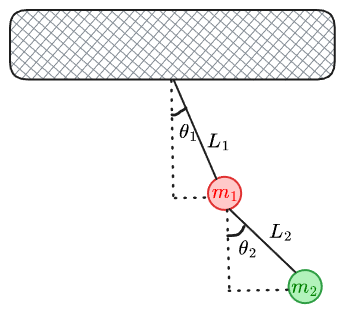
\includegraphics[scale=0.7]{figures/double_pendulum_final.png}
    \caption{Schéma d'un double pendule. Le support en gris hachuré est fixe. La masse $m_1$ est relié au support par une corde de taille fixe $L_1$. La masse $m_2$ est reliée à la masse $m_1$ par une corde de taille fixe $L_2$.}
\end{figure}

\subsubsection{Système de coordonnées généralisées}
La position en tout temps de la masse $m_1$ est donnée par l'angle $\theta_1$ et il en va de même pour la masse $m_2$ avec l'angle $\theta_2$. Les deux masses sont soumis à des contraintes: la longueur de la première corde, $L_1$, et la longueur de la seconde corde $L_2$.  Ces contraintes permettent de réécrire les coordonnées cartésiennes $(x_i, y_i)$ de ces deux masses en fonction d'une variable $\theta_i$ et de constantes connues $L_i$. Nous choisirons donc les angles $\theta_1$ et $\theta_2$ comme coordonnées généralisées. 

\noindent Réexprimons à présent $(x_1, y_1)$ en termes de $L_1$ et $\theta_1$. Pour la masse $m_1$, la contrainte est la longueur de la première corde $L_1$. On a,
\begin{align}
    x_1 &= L_1\sin (\theta_1) \label{eq:m1_double_pendulum}\\
    y_1 &= -L_1\cos(\theta_1) \, .
\end{align}

\noindent On fait la même chose à présent pour réexprimer $(x_2, y_2)$ en termes de $L_2$ et $\theta_2$. Pour la masse $m_2$, la contrainte est la longueur de la deuxième corde $L_2$. On a, 
\begin{align}
    x_2 &= x_1 + L_2\sin(\theta_2) \\
    &= L_1\sin(\theta_1) + L_2\sin(\theta_2)
        \\
    y_2 &=y_1 -L_2\cos(\theta_2)\\
    &= -L_1\cos(\theta_1)-L_2\cos(\theta_2)
\end{align}

\subsubsection{Calcul de l'énergie cinétique du système}
L'énergie cinétique totale du système est simplement l'addition de l'énergie cinétique des composantes du système, c'est-à-dire,  
\begin{align}
    K_{tot} = K_1 + K_2
\end{align}
où $K_1$ est l'énergie cinétique de la masse 1 et $K_2$ est l'énergie cinétique de la masse 2. La formule de l'énergie cinétique que vous avez sûrement vue en première ou en seconde est la suivante
\begin{align}
    K = \frac{1}{2}mv^2
\end{align}
Lorsqu'on est à des dimensions supérieures à 1, il est utile d'avoir la forme vectorielle de cette formule
\begin{align}
    K &= \frac{1}{2}m\lVert \mathbf{v}\rVert^2
    \\
    &=\frac{1}{2}m(v_x^2 + v_y^2) \label{eq:kinetic_energy}
\end{align}
où $\mathbf{v}$ est le vecteur vitesse et où $\lVert \mathbf{v}\rVert^2$ dénote la norme du vecteur vitesse, i.e. 
\begin{align}
    \lVert \mathbf{v}\rVert^2 = v_x^2 + v_y^2
\end{align}
(je m'arrête ici à deux composantes du vecteur vitesse parce qu'on a que deux dimensions dans notre problème du double pendule).
Il ne nous reste plus qu'à utiliser la formule \cref{eq:kinetic_energy} pour la masse $m_1$ pour calculer $K_1$, ensuite pour la masse $m_2$ pour calculer $K_2$ et finalement pour calculer $K_{tot} = K_1 + K_2$.

\noindent \textbf{Calcul de l'énergie cinétique de la masse 1.}

\noindent On obtient $v_{1,x}$ et $v_{1,y}$ en dérivant par rapport au temps les équations \cref{eq:m1_double_pendulum},
\begin{align}
    v_{1,x} &= \frac{d x_1}{dt} \\
    &= L_1\frac{d}{dt}\bigg[\sin (\theta_1)\bigg]
    \\
    &= L_1\frac{d }{d\theta_1}\bigg[\sin(\theta_1) \bigg]\frac{d\theta_1}{dt}
    \\
    &=L_1\cos(\theta_1)\dot{\theta}_1
\end{align}
où $\dot{\theta}_1=d\theta_1/dt$ dénote la dérivée de $\theta_1$ par rapport au temps (on parle de vitesse angulaire). On notera un peu plus tard $\omega_1\equiv \dot{\theta}_1$. On fait la même chose pour la composante verticale de la vitesse, 
\begin{align}
    v_{1,y} &= \frac{d y_1}{dt}
    \\
    &= -L_1\frac{d}{dt}\bigg[\cos(\theta_1)\bigg]
    \\
    &= -L_1 \frac{d}{d \theta_1}\bigg[\cos(\theta_1)\bigg]\frac{d \theta_1}{dt}
    \\
    &=-L_1\times (-\sin(\theta_1)) \dot{\theta}_1
    \\
    &=L_1 \sin(\theta_1)\dot{\theta}_1
\end{align}
On peut à présent calculer la norme au carré du vecteur vitesse
\begin{align}
    \lVert \mathbf{v}\rVert^2 &= v^2_{1,x} + v^2_{1,y}
    \\
    &= L_1^2\cos^2(\theta_1)\dot{\theta}_1^2 + L_1^2\sin^2(\theta_1)\dot{\theta}_1^2
    \\
    &=L_1^2\dot{\theta}_1^2\times \underbrace{[\cos^2(\theta_1) + \sin^2(\theta_1)]}_{=1}
    \\
    &= L_1^2\dot{\theta}_1^2
\end{align}

On remplace dans la formule de l'énergie cinétique et on obtient la contribution de la masse 1 à l'énergie cinétique du système, 
\begin{align}
    K_1 &= \frac{1}{2}m_1L_1^2 \dot{\theta}_1^2
\end{align}

\noindent \textbf{Calcul de l'énergie cinétique de la masse 2.}


\noindent Je vais aller un peu plus vite ici parce qu'on suit les mêmes étapes que pour le calcul de la masse $1$. 
On cherche à calculer la norme de la vitesse de la masse 2. La composante $x$ de la vitesse de la masse 2 est donnée par,
\begin{align}
    v_{x, 2} &= \frac{dx_2}{dt}\\
    &=\frac{d}{dt}\bigg[x_1 +  L_2\sin(\theta_2)\bigg]
    \\
    &=v_{x,1}+L_2\frac{d}{d\theta_2}\bigg[\sin(\theta_2)\bigg]\frac{d\theta_2}{dt}
    \\
    &=L_1\cos(\theta_1)\dot{\theta}_1 + L_2\cos(\theta_2)\dot{\theta}_2\, .
\end{align}

\noindent La composante $y$ de la vitesse de la masse 2 est donnée par, 
\begin{align}
    v_{y, 2} &= \frac{d y_2}{dt}
    \\
    &= \frac{d}{dt}\bigg[y_1 - L_2\cos(\theta_2)\bigg]
    \\
    &=v_{y, 1} - L_2\frac{d}{dt}\bigg[\cos(\theta_2)\bigg]
    \\
    &=v_{y, 1} - L_2\frac{d}{d \theta_2}\bigg[\cos(\theta_2)\bigg]\frac{d\theta_2}{dt}
    \\
    &=L_1\sin(\theta_1)\dot{\theta}_1 +L_2\sin(\theta_2)\dot{\theta}_2
\end{align}
On met maintenant au carré les deux composantes de la vitesse, 
\begin{align}
    v^2_{x, 2} &=L_1^2\cos^2(\theta_1)\dot{\theta}_1^2 + L_2^2\cos^2(\theta_2)\dot{\theta}^2_2 + 2L_1L_2\dot{\theta}_1\dot{\theta}_2\cos(\theta_1)\cos(\theta_2)
    \\
    v^2_{y, 2} &=L_1^2\sin^2(\theta_1)\dot{\theta}_1^2 + L_2^2\sin^2(\theta_2)\dot{\theta}^2_2 + 2L_1L_2\dot{\theta}_1\dot{\theta}_2\sin(\theta_1)\sin(\theta_2)
\end{align}
Maintenant, on prend une grande inspiration et on apprécie la beauté de la physique et des mathématiques. On va utiliser deux identités trigonométriques dans ce qui suit, 
\begin{align}
    \cos^2(\theta) + \sin^2(\theta)&=1\, ,
    \\
    \cos(a)\cos(b)+\sin(a)\sin(b)&=\cos(b-a)\, .
\end{align}
On obtient ainsi la norme au carré de la vitesse de la masse 2, 
\begin{align}
    \lVert \mathbf{v}_2\rVert^2 &= v_{x,2}^2 + v_{y, 2}^2\, ,\\
    &=L_1^2\dot{\theta}_1^2 + L_2^2\dot{\theta}_2^2 +2L_1L_2 \dot{\theta}_1\dot{\theta}_2\cos(\theta_2-\theta_1)\, .
\end{align}
L'énergie cinétique de la masse 2 est donc, 
\begin{align}
    K_2 = \frac{1}{2}m_2L_1^2\dot{\theta}_1^2 + \frac{1}{2}m_2L_2^2\dot{\theta}_2^2 +m_2L_1L_2 \dot{\theta}_1\dot{\theta}_2\cos(\theta_2-\theta_1)\, .
\end{align}

\noindent\textbf{Calcul de l'énergie cinétique totale du système.}

\noindent En additionnant les énergies cinétiques des deux masses du système (les cordes sont idéales et assumées sans masse), on obtient
\begin{align}
    K &=K_1 + K_2 \, ,
    \\
    &= \frac{1}{2}m_1L_1^2 \dot{\theta}_1^2+\frac{1}{2}m_2L_1^2\dot{\theta}_1^2 + \frac{1}{2}m_2L_2^2\dot{\theta}_2^2 +m_2L_1L_2 \dot{\theta}_1\dot{\theta}_2\cos(\theta_2-\theta_1)\, .
\end{align}

\subsubsection{Calcul de l'énergie potentielle}


\subsection{Dérivation d'un }

\subsection{}

\end{document}
